\documentclass[cn,10pt,math=newtx,chinesefont=founder]{elegantbook}
\title{指考物理精選}
\author{李宥頡}
\setcounter{tocdepth}{3}

%\logo{logo-blue.png}
\cover{cover.jpg}

% 本文档命令
\usepackage{array}
\newcommand{\ccr}[1]{\makecell{{\color{#1}\rule{1cm}{1cm}}}}

\definecolor{customcolor}{RGB}{32,178,170}
\colorlet{coverlinecolor}{customcolor}
\begin{document}
\maketitle
\frontmatter
\mainmatter
\chapter{指考物理題目精選}
\section{Section 1}

\begin{example}
    材質與半徑完全相同的兩金屬球分別帶有電量 Q 及 $\frac{1}{2}$Q,兩球間的距離遠大於其半徑,且兩球間的靜電作用力為 F 。今將兩球接觸後再將它們放回原來位置,
    假設過程中兩球上的總電荷守恆,則兩球間的靜電作用力變為若干?\\
    (A) $\frac{3}{2}F$ (B) $\frac{9}{8}F$ (C) $\frac{5}{4}F$ (D) $\frac{3}{4}F$ (E) $\frac{7}{8}F$\\
    \rightline{[109補考]}
\end{example}
\begin{solution}
    B
\end{solution}    
\newpage

\begin{example}
    考慮如圖5的線路,右邊是質量為$m$而長度為$l$的金屬棒,可以在導線上滑動
    形成導通的迴路,且滑動時摩擦力可忽略不計。將 整個迴路放置於量值為$B$、
    方向為射入紙面的均勻磁場中,除了電阻 R 外,假設此迴路其餘部分的電阻皆可忽略。
    如果金屬棒有一初速$v$,則經過一段特定時間 t = 0.69$\tau$ 之後,
    金屬棒的速率就會減半成$\frac{v}{2}$,而且$\tau$大致上與初速無關。其原理
    是因為電磁感應:金屬棒的運動造成迴路的磁通量改變,產生應電流, 而此電流讓運動中的金屬
    棒,在磁場中受到一反向的磁力,因此會減速,且應電流在電阻R 上會產生功率消耗。$\tau$可由時間
    的因次求得,下列何者為$\tau$的表示式?\\
    (A) $\frac{mR}{l^2 B^2}$ (B) $\frac{m^2 R}{l B^2}$ (C) $\frac{mB}{l R^2}$ (D) $\frac{mB^2}{l^2 R}$ (E) $\frac{l^2 B^2}{m R^2}$\\
    \rightline{[109補考]}
\end{example}
\begin{solution}
    A
\end{solution}
\begin{figure}[htbp]
    \flushright
    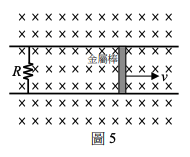
\includegraphics[width=0.3\textwidth]{109_13.png}
\end{figure}
\newpage

\begin{example}
    某生進行光電效應實驗,使用的正極板與負極板表面均為金屬鈉,其功函數為 2.3 eV,而電源提供的電位差為 3.0 V。
    通常在光電效應實驗中是將光照射在正極板上,但某生在實驗中卻將波長400 nm 的光照射在負極板上,則光電子到達正極板時
    的最大動能約為何?\\
    (A) 5.4eV (B) 3.8eV (C) 3.1eV (D) 2.3eV (E) 0.8eV \\
    \rightline{[109補考]}
\end{example}
\begin{solution}
    B
\end{solution}
\newpage

\begin{example}
    一條長為R的繩子綁住一個石塊,讓石塊一開始在鉛直面上作圓周運動,石塊的位置可由石塊−圓心連線和水
    平線夾角$\theta$表示,如圖9所示。若石塊在最低處的速率改為$\sqrt{\frac{7Rg}{2}}$,$g$為重力加速度,
    則石塊轉到何處時會脫離圖9所示之圓形虛線軌跡?\\
    (A) $\theta = 30^\circ$ (B) $\theta = 37^\circ$ (C) $\theta = 45^\circ$ (D) $\theta = 53^\circ$ (E) $\theta = 60^\circ$ \\
    \rightline{[109補考]}
\end{example}
\begin{solution}
    A
\end{solution}
\begin{figure}[htbp]
    \flushright
    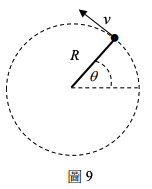
\includegraphics[width=0.3\textwidth]{109_19.png}
\end{figure}
\newpage

\begin{example}
    距離地球相當遙遠的甲、乙兩個星系因宇宙膨脹 而以$v_{a}$和$v_{b}$($v_{a}>v_{b}$)的速
    率遠離地球,若分別在兩星系上的氫原子之電子都由初始能階$E_n$躍遷到$E_m$,且$E_n$>$E_m$( n、 m為主量子數 ),
    則下列敘述哪些正確? 
    (A) 甲星系與地球的距離大於乙星系與地球的距離\\
    (B) 甲星系上的氫原子之電子由能階 $E_n$ 躍遷到 $E_m$ 時所釋放出的電磁波,在真空中以光速傳播\\
    (C) 甲星系上的氫原子之電子躍遷所釋放之電磁波到達地球時,在地球上的觀測者所測得的頻率為\\$(E_n-E_m)/h$\\
    (D) 乙星系上的氫原子之電子躍遷所釋放之電磁波到達地球時,在地球上的觀測者所測得 的波長小於$hc/(E_n-E_m)$\\
    (E) 甲、乙星系上的氫原子電子躍遷所釋放之電磁波到達地球時,在地球上的觀測者所測得來自甲星系電磁波的頻率小於來自乙星系電磁波的頻率\\
    \rightline{[109補考]}
\end{example}
\begin{solution}
    ABE
\end{solution}
\newpage

\begin{example}
    ㆒質量為 $m$ 的行星沿橢圓形軌道環繞太陽運動,已知此行星離太陽的最大和最小距離分別為 $R$ 和 $r$;行星的最小速率為 $v$ 。此行星在近日點的動能減去在遠日點的動能,其差值為何?
    \begin{enumerate}[label=(\Alph*)]
        \item 0
        \item $\frac{m(R-r)v^2}{2r}$
        \item $\frac{m(r-R)v^2}{2R}$
        \item $\frac{m(R^2-r^2)v^2}{2r^2}$
        \item $\frac{m(r^2-R^2)v^2}{2R^2}$
    \end{enumerate}
    \rightline{[92指考]}
\end{example}
\begin{solution}
    B
\end{solution}
\newpage

\begin{example}
    如圖所示,波長為$\lambda$的光子照射功函數為W的金屬表面。由正極板㆗央A點釋出的
    光電子經由電壓為$V$的平行電板作用後,最後經由負極上方的小孔B逸出。已知正
    負極板相距$L$,小孔B與負極板㆗心點相距$D$。假設小孔甚為微小,不會影響電子受
    電極的加速運動。則電子由小孔逸出時,其最大動能$K$為何?選項㆗$e>0$為電子電
    荷大小,$V>0$,$h$為卜朗克常數。
    \begin{enumerate}[label=(\Alph*)]
        \item $hc/\lambda -W-eV$
        \item $hc/\lambda -W+eV$
        \item $hc/\lambda -W-eV\frac{L}{\sqrt{L^2+D^2}}$
        \item $hc/\lambda -W+eV\frac{L}{L+D}$
        \item $hc/\lambda -W-eV\frac{D}{\sqrt{L^2+D^2}}$
    \end{enumerate}
    \rightline{[92指考]}
\end{example}
\begin{solution}
    A
\end{solution}
\begin{figure}[htbp]
    \flushright
    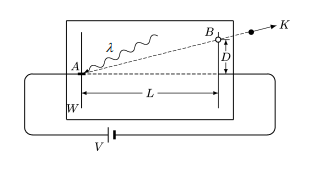
\includegraphics[width=0.4\textwidth]{image/92_10.png}
\end{figure}
\newpage

\begin{example}
    在光滑平面上的 A、B 兩圓盤,半徑均為 R,質量分別為 m 及 3m,A 盤以角速度$\omega$沿
    逆時針方向轉動, B 盤以角速度 $3\omega$ 沿順時針方向轉動, A、 B 兩盤心的連線方向為由
    西向東,且兩盤的邊緣均極光滑。今 A 盤以初速$v_0$由西向東碰撞盤心靜止的 B 盤 ,
    碰撞後 A 以$\frac{1}{2} v_0$的速度向西運動,則下列敘述哪些正確?
    \begin{enumerate}[label=(\Alph*)]
        \item 兩盤碰撞前 B 盤最南之端點(圖中b點)的速度為 $3\omega R$ ,方向向西
        \item 碰撞後, B 盤之盤心速度的量值為 $v_0$
        \item 碰撞後,B 盤最南方之端點的速度為 $3\omega R$,方向向西
        \item 碰撞後, B 盤之盤心相對於 A 盤之盤心的速度量值為 $v_0$
        \item 此兩盤碰撞前後的線動量不守恆
    \end{enumerate}
    \rightline{[92指考]}
\end{example}
\begin{solution}
    AD
\end{solution}
\begin{figure}[htbp]
    \flushright
    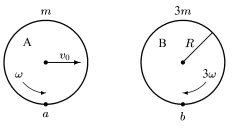
\includegraphics[width=0.3\textwidth]{image/92_14.png}
\end{figure}
\newpage

\begin{example}
    空間㆗有$-z$方向的均勻磁場 B; 在$0\leq z \leq l$的區域另有$-z$方向的均勻電場$E$。質量為
    m,電量絕對值為 q 的電荷,在$z<0$的區域,一方面向$+z$方向等速行進,一方面繞$z$
    軸做半徑為$r$的圓周運動(運動方向在$z>0$平面的投影如圖所示)。若電荷通過 $z=l$
    的平面後,運動速度的$z$分量為$z_v$ 。若地球引力的影響可以不計,則下列有關該電荷
    的敘述哪些正確?

\begin{enumerate}[label=(\Alph*)]
    \item 電荷為正
    \item 垂直於$z$軸的速度分量大小為$\frac{qBr}{m}$
    \item 在$z>l$區域時,總動能為$\frac{1}{2}mv_{z}^{2}$
    \item 在$0\leq z \leq l$的區域,磁力做功為$qv_z Bl$
    \item 在$z<0$的區域,總動能為$\frac{(qBr)^2}{2m}+\frac{1}{2}mv_{z}^{2}-qEl$
\end{enumerate}
\rightline{[92指考]}
\end{example}
\begin{solution}
    BE
\end{solution}
\begin{figure}[htbp]
    \flushright
    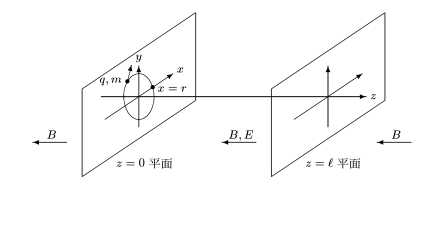
\includegraphics[width=0.5\textwidth]{image/92_20.png}
\end{figure}
\newpage

\begin{example}
    透明薄平板玻璃所組成的魚缸中,悠游著一條小魚,如圖 9 所示。在某時刻,某人沿圖㆗的 CD 直線觀
看小魚,小魚的軀幹平行於 CD 直線。下列敘述中哪些正確? 
\begin{enumerate}[label=(\Alph*)]
    \item 人所看到,魚的影像為實像。
    \item 人所看到,魚的位置和實際位置相同。
    \item 人所看到,魚的長度等於實際的長度。
    \item 當魚以速率 v,沿 CD 直線游離此人時,人所觀測到的速率小於 v。
    \item 當魚與人的位置固定時,魚缸的玻璃厚度若較大,則人所看到魚的影像比薄玻璃時更為接近。
\end{enumerate}
\rightline{[93指考]}
\end{example}
\begin{solution}
    DE
\end{solution}
\begin{figure}[htbp]
    \flushright
    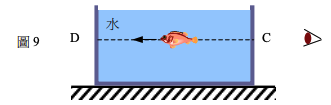
\includegraphics[width=0.5\textwidth]{image/93_13.png}
\end{figure}
\newpage
\begin{example}
    火星表面上的重力加速度比地球表面上為小。下列有關在地球和火星表面上各種物理現象的敘述,哪些
    正確? 
\begin{enumerate}[label=(\Alph*)]
    \item 繩長相同的單擺做小幅度擺動的週期相同
    \item 同一個質量-彈簧系統垂直懸掛,作簡諧振動的週期相同
    \item 同一個物體完全沒入水中所受的浮力相同
    \item 同一個物體所受的大氣浮力相同
    \item 氫原子的游離能相同
\end{enumerate}
\rightline{[93指考]}
\end{example}
\begin{solution}
    BE
\end{solution}
\newpage

\begin{example}
    質量$M$的木塊在水平地面上以初速度$v_0$滑出。已知木塊與地面間的動摩擦係數為$\mu_k$,回答下列各問題
    \begin{enumerate}
        \item 若木塊滑行一段距離$S_1$後,速度變成$\frac{v_0}{2}$,求$S_1$
        \item 試問木塊滑行多少時間(以符號$t_1$表示)後,速度由$v_0$變成$\frac{v_0}{2}$
        \item 當木塊的速度變成$\frac{v_0}{2}$的瞬間,有一質量為$m$的物體從木塊的正上方以接近零的速度落下,
        如圖12所示,並和木塊黏在一起。試問這兩個物體可繼續滑行多遠(以符號$S_2$表示)後才停住?
    \end{enumerate}
    \rightline{[93指考]}
\end{example}
\begin{figure}[htbp]
    \flushright
    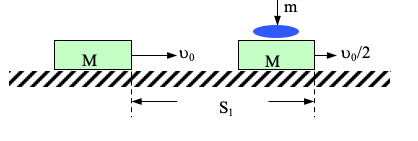
\includegraphics[width=0.5\textwidth]{image/93_n_1.png}
\end{figure}
\newpage


\begin{example}
    一質量$m$之物體以兩根頂點相距$l$的
    相同彈簧懸掛起來,兩彈簧間的夾角為$2\theta$ ($30^\circ >\theta > 20^\circ$ ),
    如圖2所示。若彈簧的自然長度亦為$l$則彈簧的力常數為何?  
    \begin{enumerate}[label=(\Alph*)]
        \item $\frac{mg}{l(cot\theta -2cos\theta)}$
        \item $\frac{mg}{l(cot\theta -2sin\theta)}$
        \item $\frac{mg}{l(tan\theta -2cos\theta)}$
        \item $\frac{mg}{l(tan\theta -2sin\theta)}$
        \item $\frac{mg}{2l sin\theta}$
    \end{enumerate}
    \rightline{[93指考補考]}
\end{example}

\begin{solution}
    A
\end{solution}
\begin{figure}[htbp]
    \flushright
    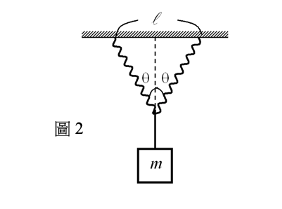
\includegraphics[width=0.5\textwidth]{image/93_c_8.png}
\end{figure}
\newpage


\begin{example}
    一粒質量為$m$的小石頭從地面上的O點以初速$v_0$ ,仰角$\theta$被射出,如圖5所示。B點為小石頭運動軌跡的最高點,
    B點與地面距離為$H$。A點則是越過最高點後的某一位置,A點與O點間的水平距離為$d$
     ($\frac{2R}{3} > d >\frac{R}{2}$ ,$R$為水平射程),
    A點與地面間的距離為$h$。若將小石頭在地面的重力位能取為零,重力加速度為$g$,且不計空氣阻力,
    則下列有關小石頭的敘述,哪些正確?
    \begin{enumerate}[label=(\Alph*)]
        \item 在A點的總力學能為$mgh$
        \item 從O點運動至A點共需時$\frac{d}{v_0}$
        \item 從O點運動至A點共需時$\frac{v_0 sin\theta}{g}+\sqrt{\frac{2(H-h)}{g}}$
        \item 在最高點B時,速度與加速度互相垂直
        \item 從O點運動至A點的過程中,重力總共作功$mgh$
    \end{enumerate}
    \rightline{[93指考補考]}
\end{example}
\begin{solution}
    CD
\end{solution}
\begin{figure}[htbp]
    \flushright
    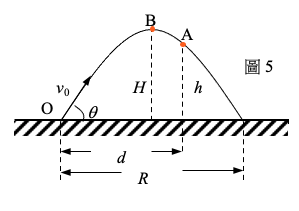
\includegraphics[width=0.5\textwidth]{image/93_c_11.png}
\end{figure}
\newpage


\begin{example}
    如圖7所示,一束波長為λ的可見光平行光束,垂直通過一條寬度$d=2\lambda$的長條形狹縫後,在遠方屏幕C上形成繞射條紋。
    若使遮闌B靠近屏幕C,且遮闌的缺口對狹縫中心O的張角$\phi$為$45^\circ$,則屏幕C上出現的亮紋對O
    的張角與下列何者最為接近?
    \begin{enumerate}[label=(\Alph*)]
        \item $15^\circ$
        \item $30^\circ$
        \item $45^\circ$
        \item $60^\circ$
        \item $75^\circ$
    \end{enumerate}
    \rightline{[94指考]}
\end{example}

\begin{solution}
    C
\end{solution}
\begin{figure}[htbp]
    \flushright
    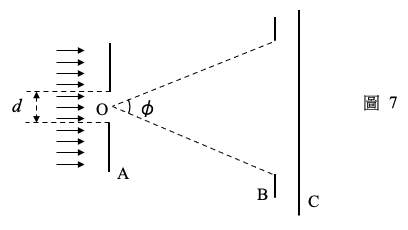
\includegraphics[width=0.5\textwidth]{image/94_7.png}
\end{figure}
\newpage

\begin{example}
    平板車在水平面上以速度 向右做等速運動,車上有一小球由板車地板上向右上方被拋出,
    如圖13所示。小球相對於板車之初速大小等於車速,方向與車速方向夾$\theta$角,且$tan\theta = \frac{4}{3}$。
    小球初速、重力加速度及車速三者位在同一平面上。小球被拋出後,因受重力影響,又落回車上。若不計空氣阻力,則下列敘述中,哪些正確
    \begin{enumerate}[label=(\Alph*)]
        \item 車內觀察者所觀測到小球的運動軌跡為一段拋物線
        \item 車外觀察者所觀測到小球的運動軌跡為一段拋物線
        \item 車外觀察者所觀測到小球停留在空中的時間較車內觀察者為短
        \item 車內觀察者所觀測到小球運動的最大高度(從地板算起),是車外觀察者的8∕3倍
        \item 車內觀察者所觀測到小球的水平位移是車外觀察者的3∕8倍
    \end{enumerate}
    \rightline{[94指考]}
\end{example}
\begin{solution}
    ABE
\end{solution}
\begin{figure}[htbp]
    \flushright
    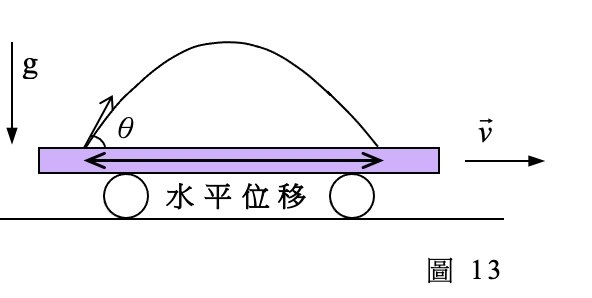
\includegraphics[width=0.5\textwidth]{image/94_14.png}
\end{figure}
\newpage

\begin{example}
    一系統由可視為質點的甲、乙兩星球組成,其質量分別為$m$與$M$ ($M > m$ ),
    在彼此間的重力作用下,分別以半徑$r$與$R$繞系統的質心O做圓周運動。
    若質心O靜止不動,兩星球相距無窮遠時,系統的總重力位能為零,則下列敘述,哪些正確?($G$為重力常數,
    亦即萬有引力常數)
    \begin{enumerate}[label=(\Alph*)]
        \item 兩星球的動量和為零
        \item 兩星球的動能為零
        \item 兩星球繞O運動的週期相等
        \item 兩星球的總重力位能為$-GmM(\frac{1}{r}+\frac{1}{R})$
        \item 兩星球的質量與繞行半徑有$mR = Mr$的關係
    \end{enumerate}
    \rightline{[94指考]}
\end{example}
\begin{solution}
    AC
\end{solution}
\newpage

\begin{example}
    下列哪些選項的因次與卜朗克常數的因次相同?
    \begin{enumerate}[label=(\Alph*)]
        \item 動量
        \item 角動量
        \item 熱量$\times$時間 
        \item 力矩$\times$時間     
        \item 電流$\times$電壓
    \end{enumerate}
    \rightline{[94指考]}
\end{example}
\begin{solution}
    BCD
\end{solution}
\newpage


%TEMPLATE
\begin{example}
    \begin{enumerate}[label=(\Alph*)]
        \item 
    \end{enumerate}
    \rightline{[指考]}
\end{example}
\begin{solution}
    
\end{solution}
\begin{figure}[htbp]
    \flushright
    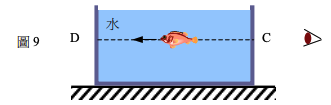
\includegraphics[width=0.5\textwidth]{image/93_13.png}
\end{figure}
\newpage


\end{document}